
Izmantotais nodomu noteikšanas modelis ir teksta klasifikators, kas sastāv no \texttt{Conv1D} un 

\texttt{MaxPooling1D} slāņiem (\textit{layers}). \texttt{Conv1D} slānis veic viendimensijas konvolūciju (\textit{convolution}), pārbīdot logu (\textit{kernel}) ar izmēru trīs pāri ievades vektoram. \texttt{MaxPooling1D} samazina modeļa parametru skaitu, izvēloties maksimālo vērtību starp diviem elementiem. Tas uzlabo modeļa ātrdarbību. Tāpat modelī ir \texttt{Dropout} slānis, kas atmet 10\% parametru, lai novērstu pārpielāgošanu. Visi modeļi tiek trenēti uz 200 epohām, jo tas ir pietiekami, lai precizitāte konverģētu uz treniņu datu kopas. Sērijas apjoms (t.i., vienlaicīgi apstrādāto piemēru skaits, \textit{batch size}) tika izvēlēts, balstoties uz datu kopas izmēra: \textit{Chatbot} datu kopai 24, \textit{Askubuntu} -- 16 un \textit{Webapps} -- 8. Apmācības ātrums (\textit{learning rate}) tika izvēlēts $10^{-3}$ \textit{Chatbot} datu kopai un $10^{-4}$ pārējām datu kopām.

Kā optimizators tiek izmantots Adam ar parametriem: \texttt{beta\_1=0.9, beta\_2=0.999, weight\_decay=0, epsilon=0, amsgrad=False, clipnorm=1.0}. Visām metodēm tiek lietots viens neironu tīkla modelis, un rezultāti ir vidējais no četrām palaišanas reizēm.


Šajā nodaļā ir izklāstīti pētījuma rezultāti, kuru mērķis ir salīdzināt dažādu lietotāju nodomu noteikšanas metožu precizitāti angļu, latviešu, krievu, igauņu un lietuviešu valodās, izmantojot mBERT un XLM-RoBERTa jēdzientelpas un dažādu valodu datus. Nodaļā rezultāti tiek analizēti pēc precizitātes (pareizi klasificēto nodomu skaits, izdalīts ar kopējo piemēru skaitu, \textit{accuracy}) un tiek apskatīti modeļu apmācības grafiki. Tāpat nodaļā ir apskatīta iegūto rezultātu ietekme uz virtuālo asistentu sistēmu izstrādi un uzlabošanu.

\ref{tab:legend} tabula sniedz pārskatu par atšķirībām starp dažādām lietotāju nodomu noteikšanai izmantotajām metodēm, pamatojoties uz apmācībā izmantoto valodu un to, vai korpuss ir bijis mašīntulkots uz angļu valodu. Papildus \ref{tab:legend2} tabulā ir īsi definēti 1a, 1b, 2a, 2b, 3a, 3b metožu atšifrējumi par piemēru ņemot latviešu valodas korpusu, ļaujot interpretēt turpmākās tabulas ar rezultātiem.


% preferably leave this
% \begin{table}[htbp]
%   \centering
%   \caption{Apkopojums galvenajām atšķirībām starp 1a, 1b, 2a, 2b, 3a, 3b metodēm attiecībā uz apmācības valodu un korpusa valodu (oriģinālvaloda vai mašīntulkojums uz angļu valodu). Alternatīvs caption: 1a, 1b, 2a, 2b, 3a, 3b metožu abreviatūru atšifrējums.}
%   % \caption{1a, 1b, 2a, 2b, 3a, 3b metožu abreviatūru atšifrējums.}
%     \begin{tabular}{lll}\toprule
%     Abreviatūra & Treniņdati & Korpusa valoda \\\midrule
%     1a    & \multicolumn{1}{l}{\multirow{2}[0]{*}{Vienā valodā}} & mašīntulkoti angļu valodā \\
%     1b    &       & oriģinālvalodā \\\midrule
%     2a    & \multicolumn{1}{l}{\multirow{2}[0]{*}{Visās valodās}} & mašīntulkoti angļu valodā \\
%     2b    &       & oriģinālvalodā \\\midrule
%     3a    & \multicolumn{1}{l}{\multirow{2}[0]{*}{Tikai angļu valodā}} & mašīntulkoti angļu valodā \\
%     3b    &       & oriģinālvalodā \\\bottomrule
%     \end{tabular}%
%   \label{tab:legend}%
% \end{table}%


% Table generated by Excel2LaTeX from sheet 'Sheet1'
\begin{table}[htbp]
  \centering
  \caption{Apkopojums galvenajām atšķirībām starp 1a, 1b, 2a, 2b, 3a, 3b metodēm attiecībā uz apmācības valodu un ievaddatu valodu.}
    \begin{tabular}{ll}\toprule
    Abreviatūra & Atšifrējums \\\midrule
    1 & Treniņdati un testa dati vienā valodā \\
    2 & Treniņdati visās valodās, testa dati vienā valodā \\
    3 & Treniņdati angļu valodā, testa dati ne-angļu valodās \\\midrule
    a & mašīntulkoti angļu valodā \\
    b & oriģinālvalodā \\\bottomrule
    \end{tabular}%
  \label{tab:legend}%
\end{table}%


% Table generated by Excel2LaTeX from sheet 'Sheet1'
\begin{table}[htbp]
  \centering
  \caption{Piemērs 1a, 1b, 2a, 2b, 3a, 3b metožu atšifrējumam latviešu valodas datiem.}
    \begin{tabular}{ll}\toprule
    Abreviatūra & Atšifrējums \\\midrule
    1a & Apmācība un testēšana uz latviešu valodas korpusa, kas mašīntulkots uz angļu valodu \\
    1b & Apmācība un testēšana uz latviešu valodas korpusa \\\midrule
    2a & Apmācība uz visām valodām, kur ne-angļu dati mašīntulkoti uz angļu valodu,\\
       & testēšana uz latviešu valodas korpusa, kas mašīntulkots uz angļu valodu \\
    2b & Apmācība uz visām valodām, testēšana uz latviešu valodas korpusa \\\midrule
    3a & Apmācība uz angļu valodas korpusa, testēšana uz latviešu valodas korpusa,\\
       & kas mašīntulkots uz angļu valodu \\
    3b & Apmācība uz angļu valodas korpusa, testēšana uz latviešu valodas korpusa \\\bottomrule
    \end{tabular}%
  \label{tab:legend2}%
\end{table}%



\section{Chatbot datu kopa}

Tabulā \ref{tab:chatbot-labels} ir sniegta informācija par unikālo nodomu skaitu  \textit{Chatbot} treniņkopā un testa kopā, kā arī to summa.

\begin{table}[htbp]
  \centering
  \caption{Unikālo nodomu skaits \textit{Chatbot} treniņkopā un testa kopā.}
    \begin{tabular}{lrrr} \toprule
    Nodoms & Treniņkopā & Testa kopā & $\Sigma$ \\\midrule
    FindConnection & 57    & 71 & 128 \\
    DepartureTime & 43    & 35 & 78 \\
    $\Sigma$ & 100    & 106 & 206 \\\bottomrule
    \end{tabular}%
  \label{tab:chatbot-labels}%
\end{table}%


Nodomu noteikšanas precizitāte \textit{Chatbot} datu kopā ir apkopota pēc izmantotā jēdzientelpu modeļa: mBERT (\ref{tab:chatbot-bert} tabula) un XLM-RoBERTa (\ref{tab:chatbot-xlm} tabula). Salīdzinot šīs jēdzientelpas, redzams, ka angļu valodā uz XLM-RoBERTa jēdzientelpām precizitāte ir augstāka, bet lietuviešu valodā -- zemāka nekā mBERT jēdzientelpām. Kopumā mBERT un XLM-RoBERTa modeļi uzrāda līdzīgus rezultātus.
% Kopumā rezultāti liecina, ka XLM-RoBERTa jēdzientelpas ir piemērotākas nodomu noteikšanai Chatbot datu kopā.

% Kopumā rezultāti liecina, ka XLM-RoBERT pārspēja mBERT lielākajā daļā scenāriju un valodu.
% Stratēģijā, kas apmāca tikai uz angļu valodas datiem un testē citā valodā:

Igauņu valodā ir vislielākais kritums stratēģijā, kas apmāca tikai uz angļu valodas datiem un testē igauņu valodā, tas atbilst paredzētajam, jo igauņu valoda ir vismazāk pārstāvēta korpusos, uz kuriem apmācīti mBERT un XLM-RoBERTa modeļi.

Lai gan intuitīvi varētu šķist, ka modelis, kas apmācīts tikai angļu valodā, slikti spēs klasificēt nodomus citā valodā, rezultāti pierāda pretējo -- 3b kolonnā redzami salīdzinoši labi rezultāti uz testa kopām latviešu, lietuviešu un igauņu valodās (74.29\% mBERT, 78.22\% XLM-RoBERTa). Tas tādēļ, ka daudzvalodu jēdzientelpas angļu datu kopās ir līdzīgas tādu pašu teikumu jēdzientelpām citās valodās. 
% Iespējams, paralēls datu korpuss palīdz, un ja angļu valodas datu kopā nodomi būtu atsķirīgā attiecībā nekā latviešu valodā, nodomu noteikšanas precizitāte latviešu valodā būtu zemāka. TODO: izskaidrot, ka 2ab notiek language transfer/Cross-lingual Representation Learning/Increased Training Data


% maz-resursu valodas iegūst no tulkošanas uz angļu valodu

% Vidēji latviešu valodas mašīntulkojums uz angļu valodu ir ar lielāku precizitāti nekā oriģinālvalodā (1ab--2ab) abās jēdzientelpās, taču krievu valodas korpusa tulkojums uz angļu valodu precizitāti zaudēja. 

Vidēji, izmantojot latviešu valodas mašīntulkojumus uz angļu valodu, var sasniegt lielāku precizitāti nekā oriģinālvalodā (1ab--2ab) abās jēdzientelpās, taču krievu valodas korpusa tulkojums uz angļu valodu precizitāti samazināja. 


1ab nodomu noteikšanas precizitātes rezultāti abās jēdzientelpās atšķiras kļūdas robežās, mBERT ir mazliet augstāki. Skatoties vidējās vērtības latviešu, lietuviešu un igauņu valodās, vislabākā metode ir apmācīt modeli uz visu valodu apvienotā korpusa, mBERT gadījumā oriģinālvalodā (2b), bet XLM-RoBERTa -- pirms tam mašīntulkojot ne-angļu valodas tekstu uz angļu valodu (2a).



Gadījumā, kad modelis apmācīts tikai uz angļu valodas korpusa, precizitāte būtiski uzlabojās testa kopu mašīntulkojot uz angļu valodu, igauņu un lietuviešu valodās precizitātei vidēji pieaugot par 30\% un 12\% attiecīgi, izņemot krievu valodu, kur precizitāte mazliet samazinās -- par 3.8\% mBERT un 1\% XLM-RoBERTa jēdzientelpām. Šo izņēmumu krievu valodā varētu izskaidrot tās salīdzinoši labā pārstāvētība korpusos, uz kuriem apmācīti mBERT un XLM-RoBERTa modeļi, salīdzinot ar latviešu, igauņu un lietuviešu valodām (\ref{fig:dataset-size} attēls).


% Maz-resursu valodās (latviešu, lietuviešu, igauņu) mašīntulkošana angļu valodā galvenokārt uzlaboja precizitāti (1ab).

Maz-resursu valodās (latviešu, lietuviešu, igauņu) precizitāte kritās ~1\% robežās apmācot uz datiem, kas mašīntulkoti angļu valodā (1ab) salīdzinot ar to valodu oriģināldatiem. Apmācot tikai uz angļu valodas datiem un testējot uz ne-angļu valodas datiem, precizitāte būtiski ieguva no testa datu mašīntulkošanas uz angļu valodu -- mBERT par
% 92.61-74.53
18.1\%, bet XLM-RoBERTa par
% 90.88-78.22
12.7\%.

% Visās valodās visstabilākā veiktspēja ir metodei, kas apmāca modeli uz visām valodām apvienotām vienā korpusā (2ab), kas nebūtiski atšķiras no tā, vai dati pirms tam ir mašīntulkoti uz angļu valodu.


% Table generated by Excel2LaTeX from sheet 'AVERAGE_chatbot_bert-base-multi'
\begin{table}[htbp]
  \centering
  \caption{Nodomu noteikšanas precizitāte uz \textit{Chatbot} datukopas ar mBERT modeli, \%}
    \begin{tabular}{lrrrrrr} \toprule
    languages & 1a & 1b & 2a & 2b & 3a & 3b \\\midrule
    en    &   --    & \cellcolor[rgb]{ .984,  .973,  .984}91.27 &   --    & \cellcolor[rgb]{ .984,  .929,  .941}89.15 &   --    & \cellcolor[rgb]{ .353,  .541,  .776}95.05 \\
    lv    & \cellcolor[rgb]{ .984,  .941,  .953}89.62 & \cellcolor[rgb]{ .502,  .647,  .831}94.34 & \cellcolor[rgb]{ .851,  .894,  .953}92.69 & \cellcolor[rgb]{ .455,  .612,  .812}94.58 & \cellcolor[rgb]{ .604,  .718,  .867}93.87 & \cellcolor[rgb]{ .984,  .871,  .882}86.08 \\
    ru    & \cellcolor[rgb]{ .984,  .976,  .988}91.51 & \cellcolor[rgb]{ .902,  .925,  .969}92.45 & \cellcolor[rgb]{ .753,  .824,  .918}93.16 & \cellcolor[rgb]{ .753,  .824,  .918}93.16 & \cellcolor[rgb]{ .902,  .925,  .969}92.45 & \cellcolor[rgb]{ .984,  .984,  .996}91.98 \\
    et    & \cellcolor[rgb]{ .984,  .957,  .969}90.57 & \cellcolor[rgb]{ .984,  .894,  .906}87.26 & \cellcolor[rgb]{ .984,  .973,  .984}91.27 & \cellcolor[rgb]{ .984,  .933,  .945}89.39 & \cellcolor[rgb]{ .902,  .925,  .969}92.45 & \cellcolor[rgb]{ .973,  .412,  .42}62.26 \\
    lt    & \cellcolor[rgb]{ .604,  .718,  .867}93.87 & \cellcolor[rgb]{ .404,  .576,  .796}94.81 & \cellcolor[rgb]{ .984,  .976,  .988}91.51 & \cellcolor[rgb]{ .553,  .682,  .847}94.10 & \cellcolor[rgb]{ .984,  .976,  .988}91.51 & \cellcolor[rgb]{ .976,  .647,  .655}74.53 \\\midrule
    avg   & \cellcolor[rgb]{ .984,  .973,  .984}91.39 & \cellcolor[rgb]{ .988,  .988,  1}92.03 & \cellcolor[rgb]{ .965,  .973,  .992}92.16 & \cellcolor[rgb]{ .98,  .984,  1}92.08 & \cellcolor[rgb]{ .875,  .91,  .961}92.57 & \cellcolor[rgb]{ .98,  .792,  .804}81.98 \\
    avg lv-lt-et & \cellcolor[rgb]{ .984,  .973,  .984}91.35 & \cellcolor[rgb]{ .969,  .973,  .992}92.14 & \cellcolor[rgb]{ .984,  .98,  .992}91.82 & \cellcolor[rgb]{ .851,  .894,  .953}92.69 & \cellcolor[rgb]{ .867,  .906,  .961}92.61 & \cellcolor[rgb]{ .976,  .643,  .651}74.29 \\\bottomrule
    \end{tabular}%
  \label{tab:chatbot-bert}%
\end{table}%


% Table generated by Excel2LaTeX from sheet 'AVERAGE_chatbot_xlm-roberta-bas'
\begin{table}[htbp]
  \centering
  \caption{Nodomu noteikšanas precizitāte uz \textit{Chatbot} datukopas ar XLM-RoBERTa modeli, \%}
    \begin{tabular}{lrrrrrr} \toprule
    languages & 1a & 1b & 2a & 2b & 3a & 3b \\\midrule
    en    &   --    & \cellcolor[rgb]{ .514,  .655,  .835}95.28 &   --    & \cellcolor[rgb]{ .514,  .655,  .835}95.28 &  --   & \cellcolor[rgb]{ .353,  .541,  .776}96.46 \\
    lv    & \cellcolor[rgb]{ .984,  .945,  .957}90.33 & \cellcolor[rgb]{ .984,  .902,  .914}88.92 & \cellcolor[rgb]{ .737,  .812,  .914}93.63 & \cellcolor[rgb]{ .639,  .745,  .878}94.34 & \cellcolor[rgb]{ .769,  .835,  .925}93.40 & \cellcolor[rgb]{ .984,  .867,  .878}87.74 \\
    ru    & \cellcolor[rgb]{ .894,  .922,  .969}92.45 & \cellcolor[rgb]{ .988,  .988,  1}91.75 & \cellcolor[rgb]{ .988,  .988,  1}91.75 & \cellcolor[rgb]{ .608,  .722,  .867}94.58 & \cellcolor[rgb]{ .957,  .969,  .992}91.98 & \cellcolor[rgb]{ .957,  .969,  .992}91.98 \\
    et    & \cellcolor[rgb]{ .984,  .89,  .902}88.44 & \cellcolor[rgb]{ .863,  .902,  .957}92.69 & \cellcolor[rgb]{ .988,  .988,  1}91.75 & \cellcolor[rgb]{ .984,  .894,  .906}88.68 & \cellcolor[rgb]{ .984,  .929,  .941}89.86 & \cellcolor[rgb]{ .973,  .412,  .42}72.17 \\
    lt    & \cellcolor[rgb]{ .984,  .953,  .965}90.57 & \cellcolor[rgb]{ .984,  .965,  .976}91.04 & \cellcolor[rgb]{ .737,  .812,  .914}93.63 & \cellcolor[rgb]{ .576,  .698,  .855}94.81 & \cellcolor[rgb]{ .984,  .918,  .929}89.39 & \cellcolor[rgb]{ .973,  .486,  .494}74.76 \\\midrule
    avg   & \cellcolor[rgb]{ .984,  .949,  .961}90.45 & \cellcolor[rgb]{ .965,  .973,  .992}91.93 & \cellcolor[rgb]{ .863,  .902,  .957}92.69 & \cellcolor[rgb]{ .749,  .82,  .918}93.54 & \cellcolor[rgb]{ .984,  .969,  .98}91.16 & \cellcolor[rgb]{ .98,  .776,  .788}84.62 \\
    avg lv-lt-et & \cellcolor[rgb]{ .984,  .929,  .941}89.78 & \cellcolor[rgb]{ .984,  .961,  .973}90.88 & \cellcolor[rgb]{ .82,  .871,  .941}93.00 & \cellcolor[rgb]{ .875,  .91,  .961}92.61 & \cellcolor[rgb]{ .984,  .961,  .973}90.88 & \cellcolor[rgb]{ .976,  .588,  .596}78.22 \\\bottomrule
    \end{tabular}%
  \label{tab:chatbot-xlm}%
\end{table}%



% Att.~\ref{fig:chatbot-bert} parāda precizitāti apmācības laikā, lietojot mBERT jēdzientelpu un treniņdatus latviešu valodā. Redzams, ka apmācības laiks (epochs) bija nepietiekams (att.~\ref{fig:chatbot-bert}, pa labi), jo trenēšanās pārtrūka pie treniņkopas precizitātes 90\%, kad vairums citos grafikos tas sasniedza 100\%. Tas vieš cerības, ka palielinot epochs skaitu 1a un 1b scenārijos, izdotos iegūt augstāku precizitāti. Mašīntulkoto datu gadījumā trenēšanās laiks bija pietiekams (att.~\ref{fig:chatbot-bert}, pa labi), un arī precizitāte uz testa kopas ir mazliet augstāka -- 91.51\% salīdzinot ar 88.67\%.


\textbf{Apmācības gaita}

\ref{fig:chatbot-bert}.~att. parāda, cik ātri palielinās precizitāte modeļa apmācības laikā, lietojot mBERT jēdzientelpu un treniņdatus latviešu valodā. Redzams, ka apmācības laiks jeb epohu skaits bija vairāk nekā pietiekams, jo modeļa precizitāte uz treniņdatiem ātri sasniedza 100\% -- vēl pirms apritēja 50 epohas. 
Līdzīga situācija novērojama \ref{fig:chatbot-bert-all}.~att., kur parādīta precizitātes attīstība apmācībai uz visām valodām.
Tas var liecināt, ka modelis tiek pārpielāgots (\textit{overfitting}), jo precizitāte uz validācijas kopas ir vienmēr mazāka, nekā uz treniņdatu kopās -- no 90\% līdz 98\% atkarībā no izvēlētās apmācības metodes.
Arī vidējā precizitāte uz testa kopas latviešu valodā nepārsniedz 95\%, kā redzams \ref{tab:chatbot-bert}.~tabulā.

Iespējams, ka modelis tiek pārpielāgots arī angļu valodas korpusam (sk. \ref{fig:chabot-bert-xlm-en}.~att.), tomēr angļu valodas gadījumā precizitāte ātri sasniedz 100\% arī validācijas datu kopai. 
Salīdzinot savā starpā jēdzientelpu modeļus, var secināt, ka mBERT (\ref{fig:chabot-bert-xlm-en}.~att., pa kreisi) nodrošina lielāku apmācības ātrumu, nekā XLM-RoBERTa (\ref{fig:chabot-bert-xlm-en}.~att., pa labi).
Šis efekts novērojams arī treniņdatiem latviešu valodā, sk. \ref{fig:chatbot-xlm}.~att., un apvienotajai treniņdatu kopai, sk. \ref{fig:chatbot-xlm-all}.~att..
Pašā trenēšanas sākumā precizitāte palielinās lēnāk XLM-RoBERTa jēdzientelpai, tomēr jau pēc 50~epohām sasniedz mBERT rezultātus -- 100\% precizitāti treniņdatu kopai un 90\%--97\% validācijas datu kopai.
Tātad, 200 epohas ir vairāk nekā pietiekams laiks darbā izveidoto modeļu apmācībai.




\begin{figure}[h] 
   \centering
   \subcaptionbox{mašīntulkoto latviešu treniņdatu kopa}{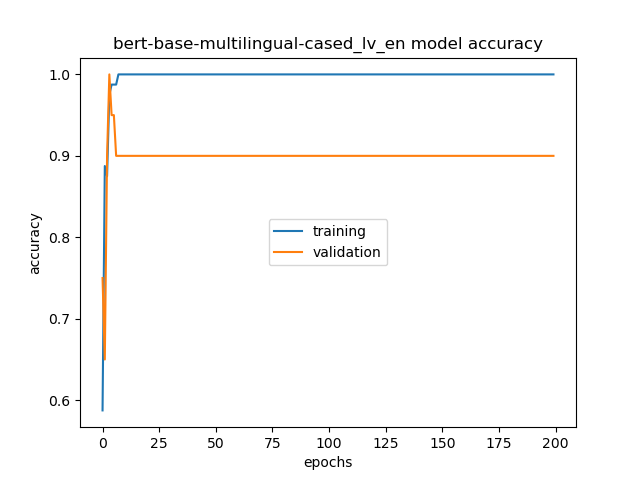
\includegraphics[width=0.49\linewidth,trim={0 0.1cm 0 0},clip]{graphs-newest/chatbot_bert-base-multilingual-cased_lv_en-accuracy.png}}
   \subcaptionbox{latviešu treniņdatu kopa}{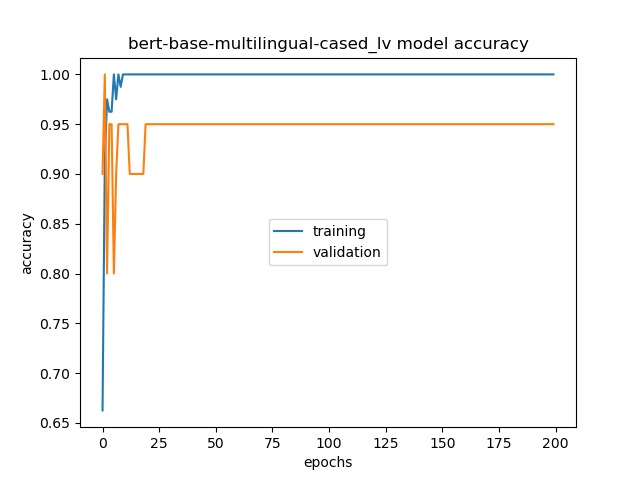
\includegraphics[width=0.49\linewidth,trim={0 0.1cm 0 0},clip]{graphs-newest/chatbot_bert-base-multilingual-cased_lv-accuracy.png}}
   \caption{Nodomu noteikšanas precizitātes palielināšanās modeļa apmācībās gaitā. Precizitāte tika aprēķināta uz treniņdatu kopas (zilā līnija) un validācijas datu kopas (oranžā līnija). Tika izmantota mBERT jēdzientelpa, \textit{Chatbot} datu kopa, apmācība un testēšana notika uz latviešu valodas korpusa (1ab metodes).} 
   \label{fig:chatbot-bert}
\end{figure}


\begin{figure}[h] 
   \centering
   \subcaptionbox{apvienotā mašīntulkoto treniņdatu kopa}{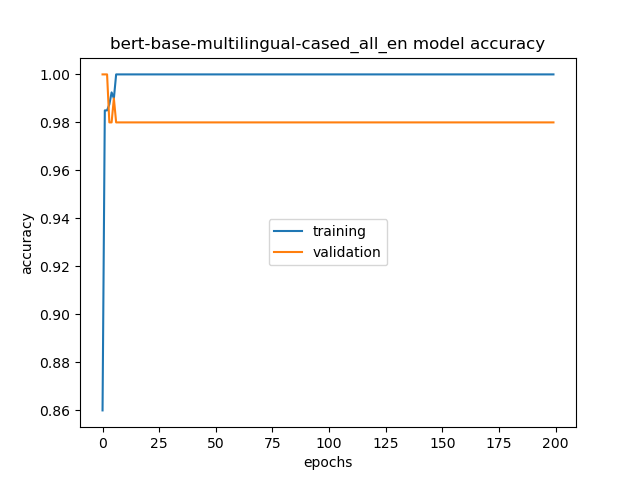
\includegraphics[width=0.49\linewidth,trim={0 0.1cm 0 0},clip]{graphs-newest/chatbot_bert-base-multilingual-cased_all_en-accuracy.png}}
   \subcaptionbox{apvienotā treniņdatu kopa}{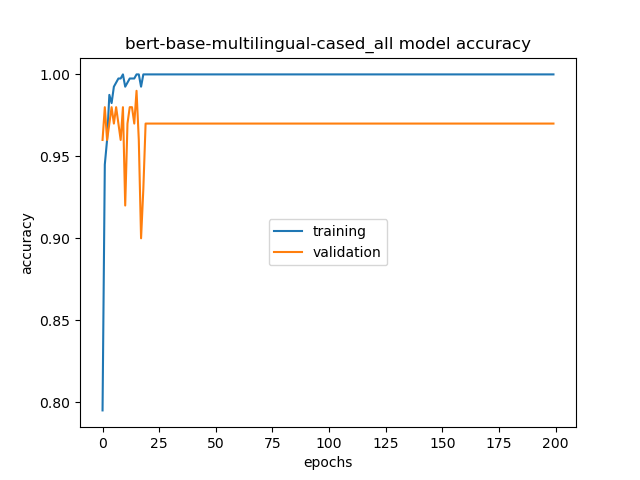
\includegraphics[width=0.49\linewidth,trim={0 0.1cm 0 0},clip]{graphs-newest/chatbot_bert-base-multilingual-cased_all-accuracy.png}}
   \caption{Nodomu noteikšanas precizitātes palielināšanās modeļa apmācībās gaitā. Precizitāte aprēķināta uz treniņdatu kopas (zilā līnija) un validācijas datu kopas (oranžā līnija). Izmantota mBERT jēdzientelpa, \textit{Chatbot} datu kopa, apmācība notika uz visām valodām, testēšana uz latviešu valodas korpusa (2ab metodes).} 
   \label{fig:chatbot-bert-all}
\end{figure}


\begin{figure}[h] 
   \centering
   \subcaptionbox{mBERT angļu treniņdatu kopa}{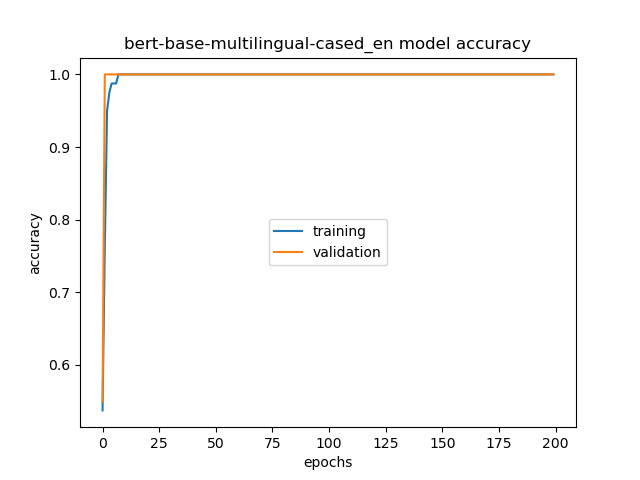
\includegraphics[width=0.49\linewidth,trim={0 0.1cm 0 0},clip]{graphs-newest/chatbot_bert-base-multilingual-cased_en-accuracy.png}}
   \subcaptionbox{XLM-RoBERTa angļu treniņdatu kopa}{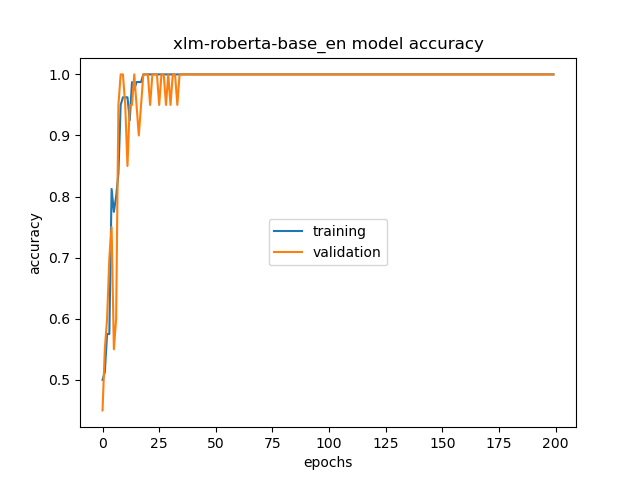
\includegraphics[width=0.49\linewidth,trim={0 0.1cm 0 0},clip]{graphs-newest/chatbot_xlm-roberta-base_en-accuracy.png}}
   \caption{Nodomu noteikšanas precizitātes palielināšanās modeļa apmācībās gaitā. Precizitāte tika aprēķināta uz treniņdatu kopas (zilā līnija) un validācijas datu kopas (oranžā līnija). Tika izmantotas dažādas jēdzientelpas, \textit{Chatbot} datu kopa, apmācība un testēšana notika uz angļu valodas korpusa (3b metode).} 
   \label{fig:chabot-bert-xlm-en}
\end{figure}


\begin{figure}[h] 
   \centering
   \subcaptionbox{mašīntulkoto latviešu treniņdatu kopa}{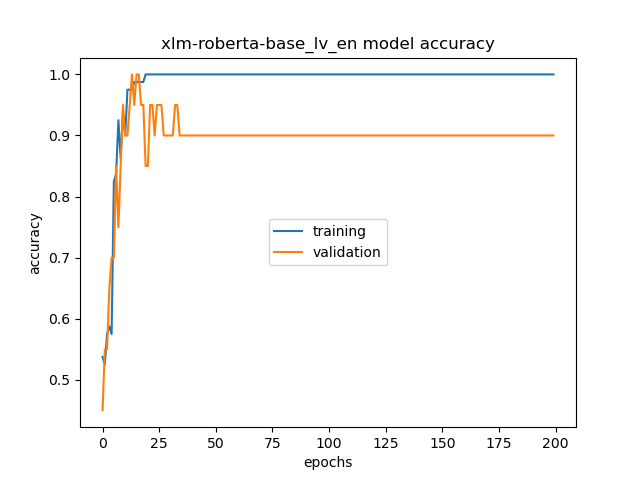
\includegraphics[width=0.49\linewidth,trim={0 0.1cm 0 0},clip]{graphs-newest/chatbot_xlm-roberta-base_lv_en-accuracy.png}}
   \subcaptionbox{latviešu treniņdatu kopa}{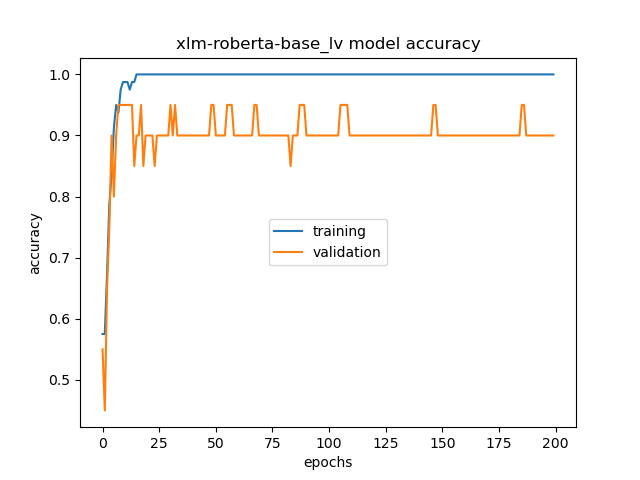
\includegraphics[width=0.49\linewidth,trim={0 0.1cm 0 0},clip]{graphs-newest/chatbot_xlm-roberta-base_lv-accuracy.png}}
   \caption{Nodomu noteikšanas precizitātes palielināšanās modeļa apmācībās gaitā. Precizitāte aprēķināta uz treniņdatu kopas (zilā līnija) un validācijas datu kopas (oranžā līnija). Izmantota XLM-RoBERTa jēdzientelpa, \textit{Chatbot} datu kopa, apmācība un testēšana notika uz latviešu valodas korpusa (1ab metodes).} 
   \label{fig:chatbot-xlm}
\end{figure}


\begin{figure}[h] 
   \centering
   \subcaptionbox{apvienotā mašīntulkoto treniņdatu kopa}{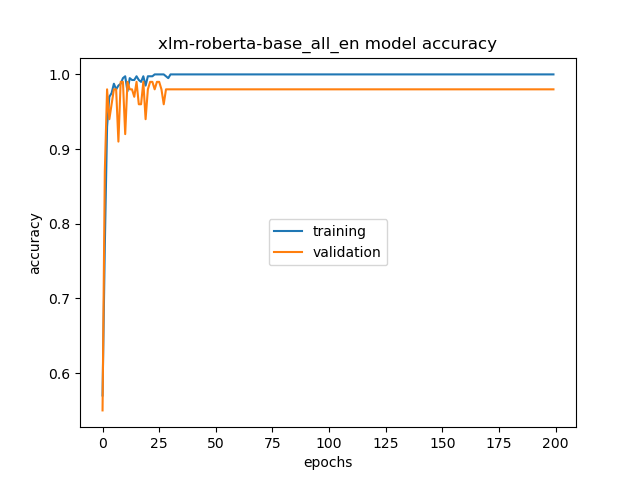
\includegraphics[width=0.49\linewidth,trim={0 0.1cm 0 0},clip]{graphs-newest/chatbot_xlm-roberta-base_all_en-accuracy.png}}
   \subcaptionbox{apvienotā treniņdatu kopa}{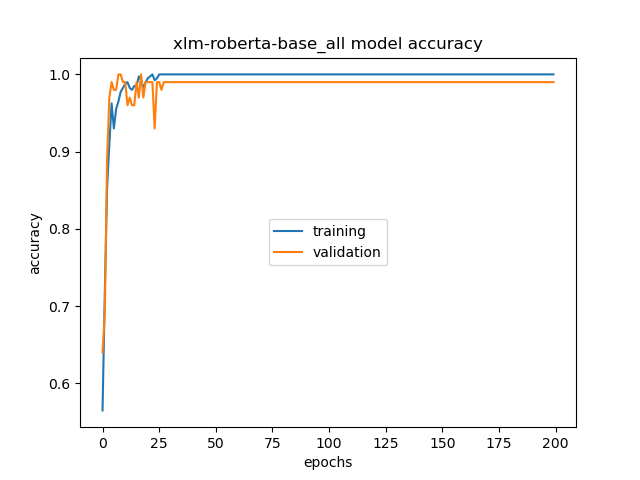
\includegraphics[width=0.49\linewidth,trim={0 0.1cm 0 0},clip]{graphs-newest/chatbot_xlm-roberta-base_all-accuracy.png}}
   \caption{Nodomu noteikšanas precizitātes palielināšanās modeļa apmācībās gaitā. Precizitāte aprēķināta uz treniņdatu kopas (zilā līnija) un validācijas datu kopas (oranžā līnija). Izmantota XLM-RoBERTa jēdzientelpa, \textit{Chatbot} datu kopa, apmācība notika uz visām valodām, testēšana uz latviešu valodas korpusa (2ab metodes).} 
   \label{fig:chatbot-xlm-all}
\end{figure}



\section{Askubuntu datu kopa}

\begin{table}[htbp]
  \centering
  \caption{Unikālo nodomu skaits “askubuntu" treniņkopā un testa kopā.}
    \begin{tabular}{lrrr} \toprule
    Nodoms & Treniņkopā & Testa kopā & $\Sigma$ \\\midrule
    Software Recommendation & 17    & 40 & 57 \\
    Make Update & 10    & 37 & 47 \\
    Shutdown Computer & 13    & 14 & 27 \\
    Setup Printer & 10    & 13 & 23\\
    None  & 3     & 5 & 8\\
   $\Sigma$ & 53    & 109 & 162 \\\bottomrule
    \end{tabular}%
  \label{tab:askubuntu-labels}%
\end{table}%



Sliktākā nodomu noteikšanas precizitāte Askubuntu datukopā ir 44.72\% (\ref{tab:askubuntu-xlm} tabula, 3b, lt), tas nozīmē, ka modelis modelis pareizi identificēs lietotāja nodomu mazāk nekā puse gadījumos. Lai gan tā ir salīdzinoši zema precizitāte, ir svarīgi atzīmēt, ka datu kopā ir pieci nodomi un, ja nodomi tiktu izvēlēti nejauši (\textit{random}), paredzamā precizitāte būtu tikai 20\%. Tāpēc modelis ar 44.72\% precizitātes līmeni joprojām darbojas ievērojami labāk nekā nejaušs.

Askubuntu datu kopā nodomu noteikšanas precizitāte ir zemāka nekā Chatbot datu kopā tādeļ, ka ir vairāk nodomu ar mazāk piemēriem katram nodomam. mBERT jēdzientelpas \textit{Askubuntu} datu kopā ir krietni pārākas par XLM-RoBERTa, tostarp angļu valodā. Attēlos redzams, ka mBERT jēdzientelpas maksimālo precizitāti sasniedz aptuveni 25 epohā, bet XLM-RoBERTa apmēram 75 epohā.

Datu kopā \textit{Askubuntu} 3b metodei ne-angļu valodās vienmēr bija viszemākā nodomu noteikšanas precizitāte gan mBERT, gan XLM-RoBERTa jēdzientelpām, tas tā ir arī pārējās datu kopās un bija sagaidāms. Turpretim vislabākā precizitāte jēdzientelpām atškiras -- mBERT tā ir 1b, bet XLM-RoBERTa 2a metode. XLM-RoBERTa gadījums parāda, ka ne pārāk labus precizitātes rezultātus (~67\%) var būtiski (par 10\%) uzlabot ar lielāku daudzvalodu korpusu.



% new table by averaging 4 runs
% Table generated by Excel2LaTeX from sheet 'AVERAGE_askubuntu_bert-base-mul'
\begin{table}[htbp]
  \centering
  \caption{Nodomu noteikšanas precizitāte uz \textit{Askubuntu} datukopas ar mBERT modeli, \%.}
    \begin{tabular}{lrrrrrr} \toprule
    languages & 1a & 1b & 2a & 2b & 3a & 3b \\\midrule
    en    &   --    & \cellcolor[rgb]{ .475,  .627,  .82}82.57 &  --     & \cellcolor[rgb]{ .357,  .545,  .78}83.26 &   --    & \cellcolor[rgb]{ .475,  .627,  .82}82.57 \\
    lv    & \cellcolor[rgb]{ .984,  .98,  .992}79.36 & \cellcolor[rgb]{ .514,  .655,  .835}82.34 & \cellcolor[rgb]{ .831,  .878,  .945}80.50 & \cellcolor[rgb]{ .514,  .655,  .835}82.34 & \cellcolor[rgb]{ .984,  .98,  .992}79.36 & \cellcolor[rgb]{ .973,  .412,  .42}54.13 \\
    ru    & \cellcolor[rgb]{ .984,  .973,  .98}78.90 & \cellcolor[rgb]{ .984,  .965,  .976}78.67 & \cellcolor[rgb]{ .984,  .902,  .914}75.92 & \cellcolor[rgb]{ .988,  .988,  1}79.59 & \cellcolor[rgb]{ .988,  .988,  1}79.59 & \cellcolor[rgb]{ .976,  .639,  .647}64.22 \\
    et    & \cellcolor[rgb]{ .753,  .824,  .918}80.96 & \cellcolor[rgb]{ .353,  .541,  .776}83.26 & \cellcolor[rgb]{ .949,  .961,  .988}79.82 & \cellcolor[rgb]{ .984,  .929,  .941}77.06 & \cellcolor[rgb]{ .91,  .933,  .973}80.05 & \cellcolor[rgb]{ .973,  .494,  .502}57.80 \\
    lt    & \cellcolor[rgb]{ .871,  .906,  .961}80.28 & \cellcolor[rgb]{ .984,  .965,  .976}78.67 & \cellcolor[rgb]{ .792,  .851,  .933}80.73 & \cellcolor[rgb]{ .984,  .941,  .949}77.52 & \cellcolor[rgb]{ .984,  .961,  .973}78.44 & \cellcolor[rgb]{ .973,  .439,  .451}55.50 \\\midrule
    avg   & \cellcolor[rgb]{ .941,  .957,  .984}79.87 & \cellcolor[rgb]{ .729,  .804,  .91}81.10 & \cellcolor[rgb]{ .984,  .98,  .992}79.24 & \cellcolor[rgb]{ .925,  .945,  .98}79.95 & \cellcolor[rgb]{ .984,  .98,  .992}79.36 & \cellcolor[rgb]{ .976,  .608,  .616}62.84 \\
    avg lv-lt-et & \cellcolor[rgb]{ .886,  .918,  .965}80.20 & \cellcolor[rgb]{ .675,  .769,  .89}81.42 & \cellcolor[rgb]{ .859,  .898,  .957}80.35 & \cellcolor[rgb]{ .984,  .973,  .984}78.98 & \cellcolor[rgb]{ .984,  .98,  .992}79.28 & \cellcolor[rgb]{ .973,  .447,  .455}55.81 \\\bottomrule
    \end{tabular}%
  \label{tab:askubuntu-bert}%
\end{table}%



% Table generated by Excel2LaTeX from sheet 'AVERAGE_askubuntu_xlm-roberta-b'
\begin{table}[htbp]
  \centering
  \caption{Nodomu noteikšanas precizitāte uz \textit{Askubuntu} datukopas ar XLM-RoBERTa modeli, \%}
    \begin{tabular}{lrrrrrr}\toprule
    languages & 1a & 1b & 2a & 2b & 3a & 3b \\\midrule
    en    &   --    & \cellcolor[rgb]{ .694,  .784,  .898}73.85 &   --    & \cellcolor[rgb]{ .353,  .541,  .776}78.90 &   --    & \cellcolor[rgb]{ .882,  .914,  .965}71.10 \\
    lv    & \cellcolor[rgb]{ .984,  .965,  .976}68.58 & \cellcolor[rgb]{ .984,  .878,  .89}64.91 & \cellcolor[rgb]{ .384,  .565,  .788}78.44 & \cellcolor[rgb]{ .557,  .686,  .851}75.92 & \cellcolor[rgb]{ .757,  .827,  .922}72.94 & \cellcolor[rgb]{ .973,  .416,  .424}44.95 \\
    ru    & \cellcolor[rgb]{ .984,  .906,  .918}66.06 & \cellcolor[rgb]{ .898,  .925,  .969}70.87 & \cellcolor[rgb]{ .51,  .651,  .831}76.61 & \cellcolor[rgb]{ .557,  .686,  .851}75.92 & \cellcolor[rgb]{ .984,  .918,  .929}66.51 & \cellcolor[rgb]{ .976,  .576,  .584}51.83 \\
    et    & \cellcolor[rgb]{ .984,  .847,  .859}63.53 & \cellcolor[rgb]{ .741,  .816,  .914}73.17 & \cellcolor[rgb]{ .557,  .686,  .851}75.92 & \cellcolor[rgb]{ .416,  .588,  .8}77.98 & \cellcolor[rgb]{ .984,  .945,  .957}67.66 & \cellcolor[rgb]{ .976,  .58,  .588}52.06 \\
    lt    & \cellcolor[rgb]{ .988,  .988,  1}69.50 & \cellcolor[rgb]{ .98,  .804,  .816}61.70 & \cellcolor[rgb]{ .447,  .608,  .812}77.52 & \cellcolor[rgb]{ .62,  .729,  .871}75.00 & \cellcolor[rgb]{ .984,  .949,  .961}67.89 & \cellcolor[rgb]{ .973,  .412,  .42}44.72 \\\midrule
    avg   & \cellcolor[rgb]{ .984,  .925,  .937}66.92 & \cellcolor[rgb]{ .984,  .973,  .984}68.90 & \cellcolor[rgb]{ .475,  .627,  .82}77.12 & \cellcolor[rgb]{ .502,  .647,  .831}76.74 & \cellcolor[rgb]{ .984,  .969,  .98}68.75 & \cellcolor[rgb]{ .976,  .6,  .612}52.94 \\
    avg lv-lt-et & \cellcolor[rgb]{ .984,  .933,  .945}67.20 & \cellcolor[rgb]{ .984,  .918,  .929}66.59 & \cellcolor[rgb]{ .463,  .62,  .816}77.29 & \cellcolor[rgb]{ .529,  .667,  .839}76.30 & \cellcolor[rgb]{ .988,  .988,  1}69.50 & \cellcolor[rgb]{ .973,  .467,  .478}47.25 \\\bottomrule
    \end{tabular}%
  \label{tab:askubuntu-xlm}%
\end{table}%



\textbf{Apmācības gaita}

\ref{fig:askubuntu-bert}.~att. parāda, ka \textit{Askubuntu} datu kopai, līdzīgi kā iepriekš aplūkotajai \textit{Chatbot} datu kopai, precizitāte uz treniņdatiem relatīvi ātri sasniedz 100\%. 
Tomēr \textit{Askubuntu} datu kopai, atšķirībā no \textit{Chatbot} datu kopas, tiek iegūta būtiski zemāka precizitāte kā validācijas datu kopai, tā arī testa kopai (sk. \ref{tab:askubuntu-bert}.~tab.).
Apmācot uz visām valodām, precizitāte uz validācijas datu kopas būtiski neuzlabojās, sk. \ref{fig:askubuntu-bert-all}.~att..
Iespējams, ka \textit{Askubuntu} datu kopai ir lielāka ievainojamība pret pārpielāgošanu, jo tajā ir lielāks nodomu skaits un mazāks piemēru skaits katram nodomam.

Salīdzinot savā starpā divus jēdzientelpu modeļus (sk. \ref{fig:askubuntu-bert-xlm-en}.~att.), var novērot, ka XLM-RoBERTa modeļa apmācība ir lēnāka -- tam ir nepieciešamas vismaz 100 epohas, salīdzinot ar 50 epohām mBERT gadījumā.
Nodomu noteikšanas modeļa trenēšanas ātrums ir līdzīgs visos XLM-RoBERTa pielietojumos, t.i. uz latviešu treniņdatiem, kā parādīts \ref{fig:askubuntu-xlm}.~att., un uz apvienotās treniņdatu kopas -- \ref{fig:askubuntu-xlm-all}.~att..

Abām jēdzientelpām var novērot, ka, lietojot apvienoto treniņdatu kopu, precizitātes vērtību apgabals uz validācijas kopas datiem sastāv no lielāka vērtību skaita, t.i., oranžās līknes lēcienveida svārstības ir mazākas.
Tas izskaidrojams ar lielāku piemēru skaitu validācijas datu kopā.




\begin{figure}[h] 
   \centering
   \subcaptionbox{mašīntulkoto latviešu treniņdatu kopa}{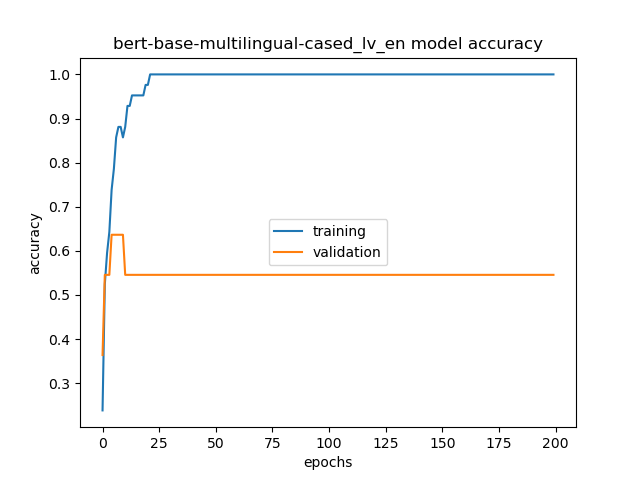
\includegraphics[width=0.49\linewidth,trim={0 0.1cm 0 0},clip]{graphs-newest/askubuntu_bert-base-multilingual-cased_lv_en-accuracy.png}}
   \subcaptionbox{latviešu treniņdatu kopa}{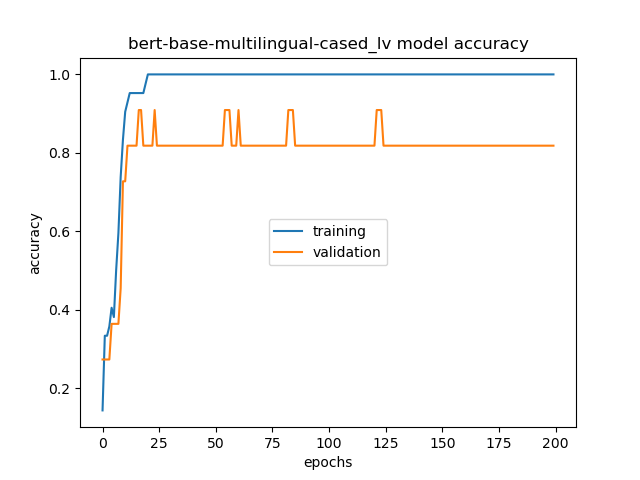
\includegraphics[width=0.49\linewidth,trim={0 0.1cm 0 0},clip]{graphs-newest/askubuntu_bert-base-multilingual-cased_lv-accuracy.png}}
   \caption{Nodomu noteikšanas precizitātes palielināšanās modeļa apmācībās gaitā. Precizitāte tika aprēķināta uz treniņdatu kopas (zilā līnija) un validācijas datu kopas (oranžā līnija). Tika izmantota mBERT jēdzientelpa, \textit{Askubuntu} datu kopa, apmācība un testēšana notika uz latviešu valodas korpusa (1ab metodes).} 
   \label{fig:askubuntu-bert}
\end{figure}


\begin{figure}[h] 
   \centering
   \subcaptionbox{apvienotā mašīntulkoto treniņdatu kopa}{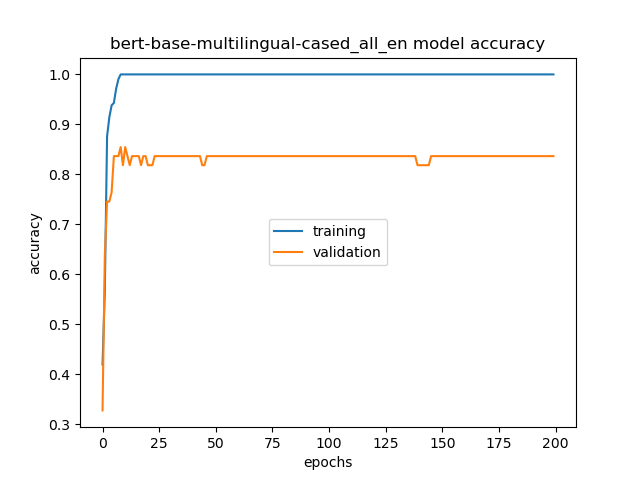
\includegraphics[width=0.49\linewidth,trim={0 0.1cm 0 0},clip]{graphs-newest/askubuntu_bert-base-multilingual-cased_all_en-accuracy.png}}
   \subcaptionbox{apvienotā treniņdatu kopa}{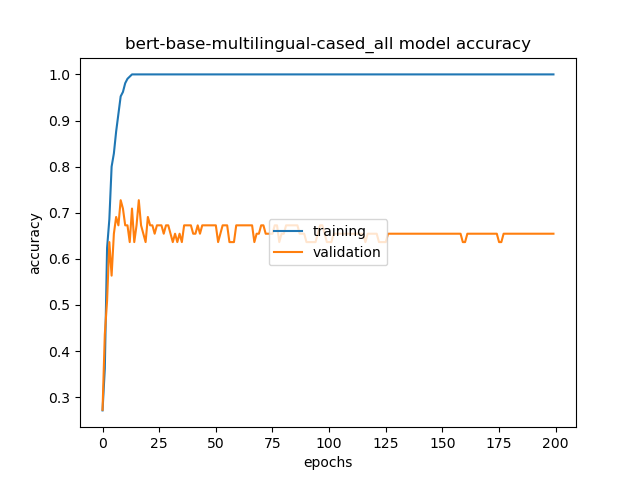
\includegraphics[width=0.49\linewidth,trim={0 0.1cm 0 0},clip]{graphs-newest/askubuntu_bert-base-multilingual-cased_all-accuracy.png}}
   \caption{Nodomu noteikšanas precizitātes palielināšanās modeļa apmācībās gaitā. Precizitāte aprēķināta uz treniņdatu kopas (zilā līnija) un validācijas datu kopas (oranžā līnija). Izmantota mBERT jēdzientelpa, \textit{Askubuntu} datu kopa, apmācība notika uz visām valodām, testēšana uz latviešu valodas korpusa (2ab metodes).} 
   \label{fig:askubuntu-bert-all}
\end{figure}


\begin{figure}[h] 
   \centering
   \subcaptionbox{mBERT angļu treniņdatu kopa}{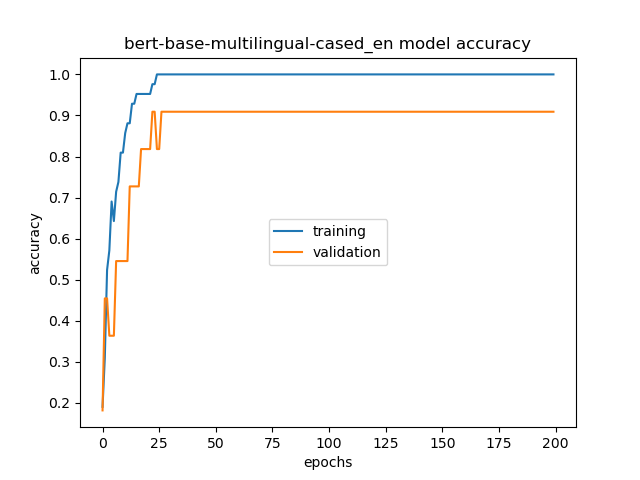
\includegraphics[width=0.49\linewidth,trim={0 0.1cm 0 0},clip]{graphs-newest/askubuntu_bert-base-multilingual-cased_en-accuracy.png}}
   \subcaptionbox{XLM-RoBERTa angļu treniņdatu kopa}{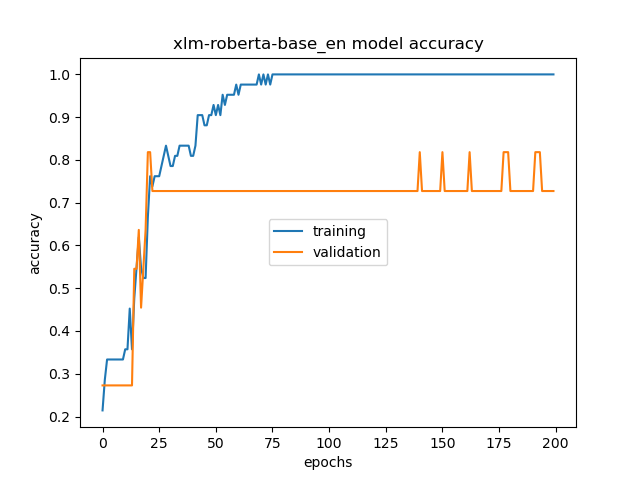
\includegraphics[width=0.49\linewidth,trim={0 0.1cm 0 0},clip]{graphs-newest/askubuntu_xlm-roberta-base_en-accuracy.png}}
   \caption{Nodomu noteikšanas precizitātes palielināšanās modeļa apmācībās gaitā. Precizitāte tika aprēķināta uz treniņdatu kopas (zilā līnija) un validācijas datu kopas (oranžā līnija). Tika izmantotas dažādas jēdzientelpas, \textit{Askubuntu} datu kopa, apmācība un testēšana notika uz angļu valodas korpusa (3b metode).} 
   \label{fig:askubuntu-bert-xlm-en}
\end{figure}


\begin{figure}[h] 
   \centering
   \subcaptionbox{mašīntulkoto latviešu treniņdatu kopa}{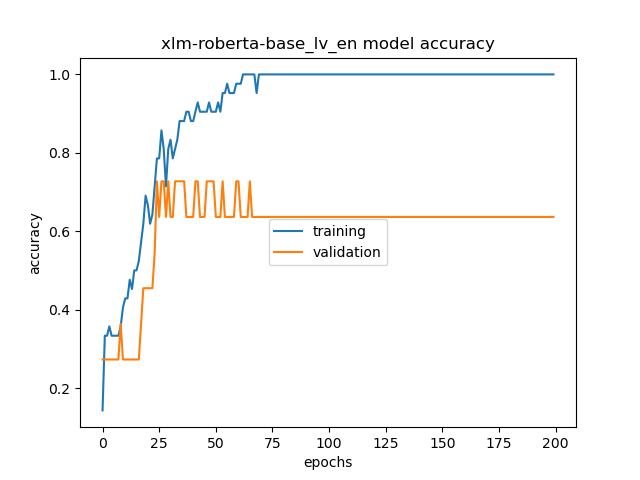
\includegraphics[width=0.49\linewidth,trim={0 0.1cm 0 0},clip]{graphs-newest/askubuntu_xlm-roberta-base_lv_en-accuracy.png}}
   \subcaptionbox{latviešu treniņdatu kopa}{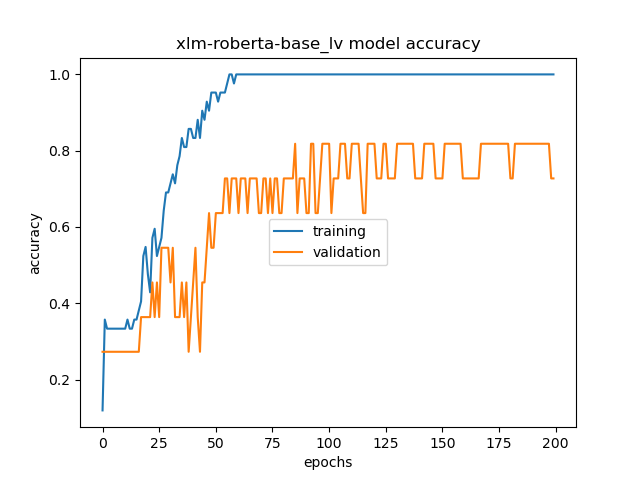
\includegraphics[width=0.49\linewidth,trim={0 0.1cm 0 0},clip]{graphs-newest/askubuntu_xlm-roberta-base_lv-accuracy.png}}
   \caption{Nodomu noteikšanas precizitātes palielināšanās modeļa apmācībās gaitā. Precizitāte aprēķināta uz treniņdatu kopas (zilā līnija) un validācijas datu kopas (oranžā līnija). Izmantota XLM-RoBERTa jēdzientelpa, \textit{Askubuntu} datu kopa, apmācība un testēšana notika uz latviešu valodas korpusa (1ab metodes).} 
   \label{fig:askubuntu-xlm}
\end{figure}


\begin{figure}[h] 
   \centering
   \subcaptionbox{apvienotā mašīntulkoto treniņdatu kopa}{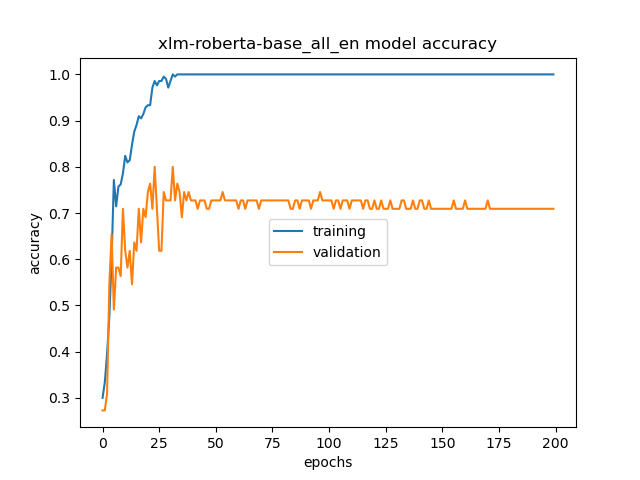
\includegraphics[width=0.49\linewidth,trim={0 0.1cm 0 0},clip]{graphs-newest/askubuntu_xlm-roberta-base_all_en-accuracy.png}}
   \subcaptionbox{apvienotā treniņdatu kopa}{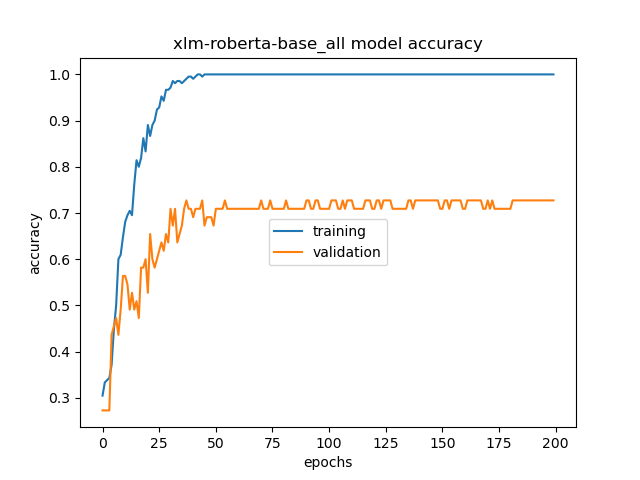
\includegraphics[width=0.49\linewidth,trim={0 0.1cm 0 0},clip]{graphs-newest/askubuntu_xlm-roberta-base_all-accuracy.png}}
   \caption{Nodomu noteikšanas precizitātes palielināšanās modeļa apmācībās gaitā. Precizitāte aprēķināta uz treniņdatu kopas (zilā līnija) un validācijas datu kopas (oranžā līnija). Izmantota XLM-RoBERTa jēdzientelpa, \textit{Askubuntu} datu kopa, apmācība notika uz visām valodām, testēšana uz latviešu valodas korpusa (2ab metodes).} 
   \label{fig:askubuntu-xlm-all}
\end{figure}



\section{Webapps datu kopa}


Webapps datu kopā ir nodoms ar tikai vienu piemēru, kas izraisa kļūdu “ValueError: The least populated class in y has only 1 member, which is too few. The minimum number of groups for any class cannot be less than 2." Tāpēc nodomi ar mazāk nekā trīs piemēriem tika apvienoti vienā nodomā “Other". Tas atbilst reālam pielietojumam industrijā, kur nodomi nav vienlīdzīgi pārstāvēti  -- piemēram, starp 115 dažādiem nodomiem divi visbiežākie nodomi kopā pārstāv 33\% datu kopas \cite{paikens2020} -- un ir svarīgi spēt atsijāt nodomus, kurus jāapstrādā klientu apkalpošanas speciālistam -- cilvēkam.

% , bet visaugstākajos rezultātos -- 2a un 2b metodēs XLM-RoBERTa ir pārāks. Šajā gadījumā spēja vienā metodē sasniegt konsekventi labus rezultātus ir svarīgāka nekā viduvēji rezultāti visās, jo pastāv iespēja izvēlēties un lietot vislabāko.


Nodomu noteikšanas precizitāte \textit{Webapps} datu kopā ir apkopota pēc izmantotā jēdzientelpu modeļa: mBERT (\ref{tab:webapps-bert} tabula) un XLM-RoBERTa (\ref{tab:webapps-xml} tabula). Salīdzinot abas tabulas, redzams, ka XLM-RoBERTa jēdzientelpām vairumā gadījumu ir zemāka preciztāte nekā nekā mBERT. Tāpat kā \textit{Askubuntu} datu kopā, arī šeit XLM-RoBERTa jēdzientelpas ļoti iegūst no lielāka daudzvalodu datu korpusa -- no 1ab un 3a vidējās 47\% precizitātes, 2ab tā pieaug par 19\%. 


%Angļu valodā 1b XLM-RoBERTa ir ar precizitāti 42.37\%, kas varētu būt nejaušība, jo 3b arī apmāca un trenē uz tieši tāda paša korpusa un ir 64.41\%, tāpēc to var neņemt vērā. Ar mBERT jēdzientelpu šāda problēma angļu valodai nebija novērota (apmācot modeli ar 1b metodi tika iegūta precizitāte 64.41\%).

Atšķirībā no pārējām datu kopām nodomu noteikšanas precizitāte igauņu valodā nav sliktāka, salīdzinot ar citām maz-resursu valodām -- igauņu valodai maksimālā precizitāte sasniedz gandrīz 75\%, bet latviešu un lietuviešu valodām tā ir attiecīgi 73\% un 80\%. Tādā veidā maz-resursu valodas uz šīs datu kopas ir ar līdzīgu precizitāti kā krievu valodai, kura ir daudz plašāk pārstāvēta tekstu korpusos.

Jāpievērš uzmanība, ka 1b un 3b tieši angļu valodā faktiski ir viena un tā pati metode -- modelis tiek trenēts uz angļu valodas treniņdatiem un testēts uz angļu valodas testa datiem, tas attiecas uz visām datu kopām. Izvēle atstāt 1b un 3b metodi atsevišķi, nevis apkopot, tika izdarīta, lai visām valodām būtu vienāds skaits eksperimentu un atklātības (\textit{transparency}) dēļ. Mašīnmācīsanās nav deterministiska. Apmācot modeli ar vienādu arhitektūru uz tiem pašiem apmācības datiem, katru reizi var iegūt atšķirīgus rezultātus apmācības procesam raksturīgās nejaušības dēļ. Modeļa svari tiek inicializēti nejauši, un apmācības laikā optimizācijas algoritms var konverģēt uz dažādiem lokāliem minimumiem, kas noved pie dažādām nodomu noteikšanas precizitātēm. Darbā tas tika ņemts vērā palaižot modeli četras reizes un izmantojot vidējo vērtību.



Webapps datu kopā uz XLM-RoBERTa jēdzientelpām 1b un 3b atšķiras par 
% 58.05-50.85
7.2\% (\ref{tab:webapps-xml} tabula). Plašāk attēlojot katras modeļa palaišanas reizes rezultātus (\ref{tab:13b-webapps} tabula) redzams, ka vidējais rezultāts apkopojot visus 1b un 3b rezultātus ir 54.45\%. Uzskatot pirmās palaišanas reizes rezultātus par netipisku vērtību (\textit{outlier}), vidējie rezultāti ir 53.67\% un 55.93\% attiecīgi. Pārējās datu kopās (\ref{tab:13b-webapps} tabula) atšķirības ir mazākas.

% average(52.54, 55.93, 52.54) = 53.67
% average(61.02, 55.93, 50.85) = 55.93


% Table generated by Excel2LaTeX from sheet '3_webapps_xlm-roberta-base_resu'
\begin{table}[htbp]
  \centering
  \caption{\textit{Webapps} datu kopa, XLM-RoBERTa jēdzientelpa precizitātes rādītāji 1b un 3b metodē angļu valodā.}
    \begin{tabular}{lcc}\toprule
    run   & 1b & 3b \\\midrule
    1 & 42.37 & 64.41 \\
    2 & 52.54 & 61.02 \\
    3 & 55.93 & 55.93 \\
    4 & 52.54 & 50.85 \\\midrule
    avg   & 50.85 & 58.05 \\
    avg all & \multicolumn{2}{c}{54.45} \\\bottomrule
    \end{tabular}%
  \label{tab:13b-webapps}%
\end{table}%



% \begin{table}[htbp]
%   \centering
%   \caption{\textit{Chatbot} un \textit{Askubuntu} datu kopas, XLM-RoBERTa jēdzientelpa angļu valodas precizitātes rādītāji 1b un 3b metodē.}
%     \begin{tabular}{|l|cc|cc|cc|cc|} \toprule
%           & \multicolumn{4}{c|}{Chatbot}   & \multicolumn{4}{c|}{Askubuntu} \\
%           & \multicolumn{2}{c|}{mBERT} & \multicolumn{2}{c|}{XLM-RoBERTa} & \multicolumn{2}{c|}{mBERT} & \multicolumn{2}{c|}{XLM-RoBERTa} \\
%     run   & \multicolumn{1}{c}{1b} & \multicolumn{1}{c|}{3b} & \multicolumn{1}{c}{1b} & \multicolumn{1}{c|}{3b} & \multicolumn{1}{c}{1b} & \multicolumn{1}{c|}{3b} & \multicolumn{1}{c}{1b} & \multicolumn{1}{c|}{3b} \\\midrule
%     1     & 91.51 & 95.28 & 95.28 & 96.23 & 78.90 & 82.57 & 77.06 & 70.64 \\
%     2     & 90.57 & 96.23 & 95.28 & 96.23 & 83.49 & 82.57 & 72.48 & 69.72 \\
%     3     & 91.51 & 94.34 & 95.28 & 96.23 & 87.16 & 79.82 & 73.39 & 74.31 \\
%     4     & 91.51 & 94.34 & 95.28 & 97.17 & 80.73 & 85.32 & 72.48 & 69.72 \\\midrule
%     avg   & 91.27 & 95.05 & 95.28 & 96.46 & 82.57 & 82.57 & 73.85 & 71.10 \\
%     avg all & \multicolumn{2}{c|}{93.16} & \multicolumn{2}{c|}{95.87} & \multicolumn{2}{c|}{82.57} & \multicolumn{2}{c|}{72.48} \\\bottomrule
%     \end{tabular}%
%   \label{tab:13b}%
% \end{table}%



\begin{table}[htbp]
  \centering
  \caption{\textit{Chatbot} un \textit{Askubuntu} datu kopas, mBERT un XLM-RoBERTa jēdzientelpu precizitātes rādītāji 1b un 3b metodē angļu valodā.}
    \begin{tabular}{l|cc|cc|cc|cc} \toprule
          & \multicolumn{4}{c|}{Chatbot}   & \multicolumn{4}{c}{Askubuntu} \\\midrule
          & \multicolumn{2}{c|}{mBERT} & \multicolumn{2}{c|}{XLM-RoBERTa} & \multicolumn{2}{c|}{mBERT} & \multicolumn{2}{c}{XLM-RoBERTa} \\
    run   & \multicolumn{1}{c}{1b} & \multicolumn{1}{c|}{3b} & \multicolumn{1}{c}{1b} & \multicolumn{1}{c|}{3b} & \multicolumn{1}{c}{1b} & \multicolumn{1}{c|}{3b} & \multicolumn{1}{c}{1b} & \multicolumn{1}{c}{3b} \\\midrule
    1     & 91.51 & 95.28 & 95.28 & 96.23 & 78.90 & 82.57 & 77.06 & 70.64 \\
    2     & 90.57 & 96.23 & 95.28 & 96.23 & 83.49 & 82.57 & 72.48 & 69.72 \\
    3     & 91.51 & 94.34 & 95.28 & 96.23 & 87.16 & 79.82 & 73.39 & 74.31 \\
    4     & 91.51 & 94.34 & 95.28 & 97.17 & 80.73 & 85.32 & 72.48 & 69.72 \\\midrule
    avg   & 91.27 & 95.05 & 95.28 & 96.46 & 82.57 & 82.57 & 73.85 & 71.10 \\
    avg all & \multicolumn{2}{c|}{93.16} & \multicolumn{2}{c|}{95.87} & \multicolumn{2}{c|}{82.57} & \multicolumn{2}{c}{72.48} \\\bottomrule
    \end{tabular}%
  \label{tab:13b}%
\end{table}%




\begin{table}[htbp]
  \centering
  \caption{Unikālo nodomu skaits ``webapps" treniņkopā un testa kopā. Ar treknrakstu iezīmētas nodomi, kuri ir pietiekami pārstāvētas, pārējie nodomi tika apvienoti vienā jaunā nodomā: “Other"}
    \begin{tabular}{lrrr} \toprule
    Nodoms & Treniņkopā & Testa kopā & $\Sigma$ \\\midrule
    \textbf{Find Alternative} & \textbf{7} & \textbf{16} & 23\\
    \textbf{Delete Account} & \textbf{7} & \textbf{10} & 17\\
    \textbf{Filter Spam} & \textbf{6} & \textbf{14} & 20 \\
    \textbf{Sync Accounts} & \textbf{3} & \textbf{6} & 9 \\
    Change Password & 2     & 6 & 8\\
    None  & 2     & 4 & 6\\
    Export Data & 2     & 3 & 5 \\
    Download Video & 1     & 0 & 1\\
    $\Sigma$ & 30    & 59 & 89 \\\bottomrule
    \end{tabular}%
  \label{tab:webapps-labels}%
\end{table}%


% Table generated by Excel2LaTeX from sheet 'AVERAGE_webapps_bert-base-multi'
\begin{table}[htbp]
  \centering
  \caption{Nodomu noteikšanas precizitāte uz \textit{Webapps} datukopas ar mBERT modeli, \%.}
    \begin{tabular}{lrrrrrr}\toprule
    languages & 1a & 1b & 2a & 2b & 3a & 3b \\\midrule
    en    &  --   & \cellcolor[rgb]{ .843,  .886,  .949}66.53 &   --    & \cellcolor[rgb]{ .941,  .957,  .984}64.83 &   --    & \cellcolor[rgb]{ .984,  .969,  .98}63.14 \\
    lv    & \cellcolor[rgb]{ .698,  .784,  .898}69.07 & \cellcolor[rgb]{ .984,  .953,  .965}62.29 & \cellcolor[rgb]{ .576,  .698,  .855}71.19 & \cellcolor[rgb]{ .867,  .906,  .961}66.10 & \cellcolor[rgb]{ .984,  .961,  .973}62.71 & \cellcolor[rgb]{ .973,  .412,  .42}33.47 \\
    ru    & \cellcolor[rgb]{ .82,  .871,  .941}66.95 & \cellcolor[rgb]{ .722,  .8,  .906}68.64 & \cellcolor[rgb]{ .353,  .541,  .776}75.00 & \cellcolor[rgb]{ .502,  .647,  .831}72.46 & \cellcolor[rgb]{ .984,  .961,  .973}62.71 & \cellcolor[rgb]{ .976,  .62,  .627}44.49 \\
    et    & \cellcolor[rgb]{ .984,  .914,  .925}60.17 & \cellcolor[rgb]{ .984,  .898,  .91}59.32 & \cellcolor[rgb]{ .38,  .561,  .788}74.58 & \cellcolor[rgb]{ .867,  .906,  .961}66.10 & \cellcolor[rgb]{ .965,  .973,  .992}64.41 & \cellcolor[rgb]{ .973,  .506,  .514}38.56 \\
    lt    & \cellcolor[rgb]{ .984,  .961,  .973}62.71 & \cellcolor[rgb]{ .984,  .89,  .902}58.90 & \cellcolor[rgb]{ .525,  .663,  .839}72.03 & \cellcolor[rgb]{ .82,  .871,  .941}66.95 & \cellcolor[rgb]{ .984,  .929,  .941}61.02 & \cellcolor[rgb]{ .973,  .42,  .427}33.90 \\\midrule
    avg   & \cellcolor[rgb]{ .949,  .961,  .988}64.72 & \cellcolor[rgb]{ .984,  .969,  .98}63.14 & \cellcolor[rgb]{ .459,  .616,  .816}73.20 & \cellcolor[rgb]{ .8,  .855,  .933}67.29 & \cellcolor[rgb]{ .984,  .961,  .973}62.71 & \cellcolor[rgb]{ .976,  .584,  .592}42.71 \\
    avg lv-lt-et & \cellcolor[rgb]{ .988,  .988,  1}63.98 & \cellcolor[rgb]{ .984,  .914,  .925}60.17 & \cellcolor[rgb]{ .494,  .639,  .827}72.60 & \cellcolor[rgb]{ .851,  .894,  .953}66.38 & \cellcolor[rgb]{ .984,  .961,  .973}62.71 & \cellcolor[rgb]{ .973,  .443,  .451}35.31 \\\bottomrule
    \end{tabular}%
  \label{tab:webapps-bert}%
\end{table}%


% Table generated by Excel2LaTeX from sheet 'AVERAGE_webapps_xlm-roberta-bas'
\begin{table}[htbp]
  \centering
  \caption{Nodomu noteikšanas precizitāte uz \textit{Webapps} datukopas ar XLM-RoBERTa modeli, \%.}
    \begin{tabular}{lrrrrrr}\toprule
    languages & 1a & 1b & 2a & 2b & 3a & 3b \\\midrule
    en    &   --    & \cellcolor[rgb]{ .965,  .973,  .992}50.85 &  --   & \cellcolor[rgb]{ .475,  .627,  .82}66.53 &   --    & \cellcolor[rgb]{ .737,  .812,  .914}58.05 \\
    lv    & \cellcolor[rgb]{ .976,  .659,  .671}37.29 & \cellcolor[rgb]{ .988,  .988,  1}50.00 & \cellcolor[rgb]{ .463,  .62,  .816}66.95 & \cellcolor[rgb]{ .353,  .541,  .776}70.34 & \cellcolor[rgb]{ .984,  .843,  .855}44.49 & \cellcolor[rgb]{ .973,  .455,  .463}29.24 \\
    ru    & \cellcolor[rgb]{ .98,  .769,  .78}41.53 & \cellcolor[rgb]{ .949,  .961,  .988}51.27 & \cellcolor[rgb]{ .541,  .675,  .843}64.41 & \cellcolor[rgb]{ .608,  .722,  .867}62.29 & \cellcolor[rgb]{ .98,  .835,  .843}44.07 & \cellcolor[rgb]{ .976,  .573,  .58}33.90 \\
    et    & \cellcolor[rgb]{ .976,  .659,  .671}37.29 & \cellcolor[rgb]{ .984,  .898,  .91}46.61 & \cellcolor[rgb]{ .525,  .663,  .839}64.83 & \cellcolor[rgb]{ .502,  .647,  .831}65.68 & \cellcolor[rgb]{ .984,  .933,  .945}47.88 & \cellcolor[rgb]{ .973,  .486,  .494}30.51 \\
    lt    & \cellcolor[rgb]{ .725,  .804,  .91}58.47 & \cellcolor[rgb]{ .984,  .922,  .933}47.46 & \cellcolor[rgb]{ .396,  .573,  .792}69.07 & \cellcolor[rgb]{ .502,  .647,  .831}65.68 & \cellcolor[rgb]{ .737,  .812,  .914}58.05 & \cellcolor[rgb]{ .973,  .412,  .42}27.54 \\\midrule
    avg   & \cellcolor[rgb]{ .98,  .824,  .835}43.64 & \cellcolor[rgb]{ .984,  .969,  .976}49.24 & \cellcolor[rgb]{ .482,  .631,  .824}66.31 & \cellcolor[rgb]{ .486,  .635,  .824}66.10 & \cellcolor[rgb]{ .984,  .949,  .961}48.62 & \cellcolor[rgb]{ .976,  .624,  .631}35.85 \\
    avg lv-lt-et & \cellcolor[rgb]{ .98,  .843,  .851}44.35 & \cellcolor[rgb]{ .984,  .937,  .945}48.02 & \cellcolor[rgb]{ .463,  .62,  .816}66.95 & \cellcolor[rgb]{ .451,  .612,  .812}67.23 & \cellcolor[rgb]{ .984,  .988,  1}50.14 & \cellcolor[rgb]{ .973,  .451,  .459}29.10 \\\bottomrule
    \end{tabular}%
  \label{tab:webapps-xml}%
\end{table}%



\textbf{Apmācības gaita}

Līdzīgi kā \textit{Askubuntu} datu kopai, \textit{Webapps} datu kopai apmācības precizitāte ātri pieaug līdz 100\%, bet validācijas precizitāte ir ierobežota, un tās svārstības pat ir lielākas, jo piemēru skaits uz vienu nodomu ir mazāks. 
Precizitātes attīstība laikā ir parādīta \ref{fig:webapps-bert}.~att. (treniņdati latviešu valodā) un \ref{fig:webapps-bert-all}. (apvienotā treniņdatu kopa).
Tiek vēlreiz apstiprināts arī secinājums par to, ka XLM-RoBERTa gadījumā apmācības ātrums ir zemāks par ātrumu mBERT gadījumā, kā parādīts \ref{fig:webapps-bert-xlm-en}.~att. treniņdatiem angļu valodā.

\ref{fig:webapps-xlm}.~attēls parāda precizitātes attīstību modeļiem, kas izmanto XLM-RoBERTa jēdzientelpu un latviešu treniņdatus (pa labi) vai mašīntulkotos latviešu treniņdatus (pa kreisi).
Iespējams, ka ar XLM-RoBERTa precizitāte latviešu treniņdatu gadījumā ir īpaši zema \textit{Webapps} datukopas īpatnību dēļ, jo ļoti zema vidējā precizitāte ir novērota arī krievu un igauņu valodām, sk. \ref{tab:webapps-xml}.~tab..
Savukārt \ref{fig:webapps-xlm-all}.~att. demonstrē, ka mašīntulkošanas ietekme uz precizitāti ir ļoti maza gadījumā, kad izmantota apvienotā treniņdatu kopa no visām valodām.


\begin{figure}[h] 
   \centering
   \subcaptionbox{mašīntulkoto latviešu treniņdatu kopa}{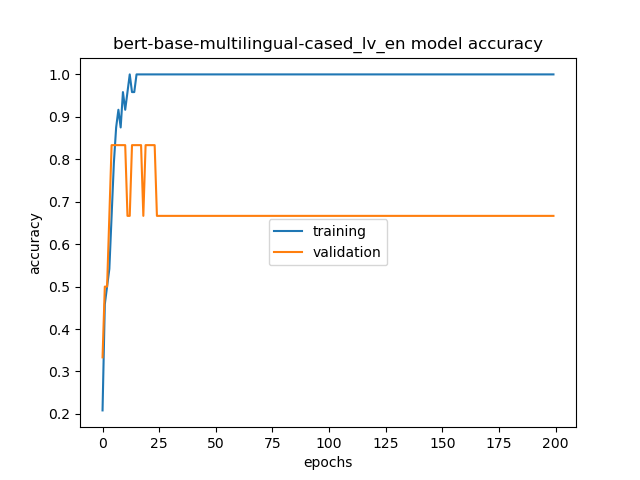
\includegraphics[width=0.49\linewidth,trim={0 0.1cm 0 0},clip]{graphs-newest/webapps_bert-base-multilingual-cased_lv_en-accuracy.png}}
   \subcaptionbox{latviešu treniņdatu kopa}{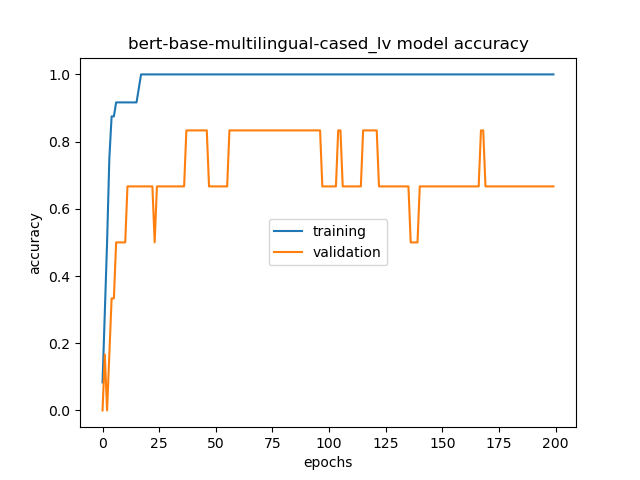
\includegraphics[width=0.49\linewidth,trim={0 0.1cm 0 0},clip]{graphs-newest/webapps_bert-base-multilingual-cased_lv-accuracy.png}}
   \caption{Nodomu noteikšanas precizitātes palielināšanās modeļa apmācībās gaitā. Precizitāte tika aprēķināta uz treniņdatu kopas (zilā līnija) un validācijas datu kopas (oranžā līnija). Tika izmantota mBERT jēdzientelpa, \textit{Webapps} datu kopa, apmācība un testēšana notika uz latviešu valodas korpusa (1ab metodes).} 
   \label{fig:webapps-bert}
\end{figure}


\begin{figure}[h] 
   \centering
   \subcaptionbox{apvienotā mašīntulkoto treniņdatu kopa}{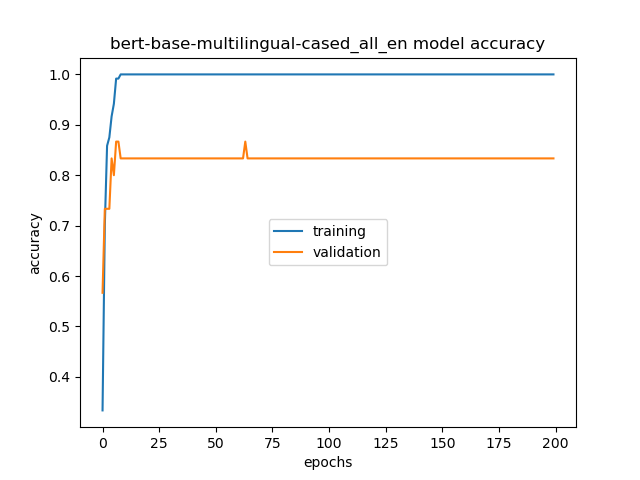
\includegraphics[width=0.49\linewidth,trim={0 0.1cm 0 0},clip]{graphs-newest/webapps_bert-base-multilingual-cased_all_en-accuracy.png}}
   \subcaptionbox{apvienotā treniņdatu kopa}{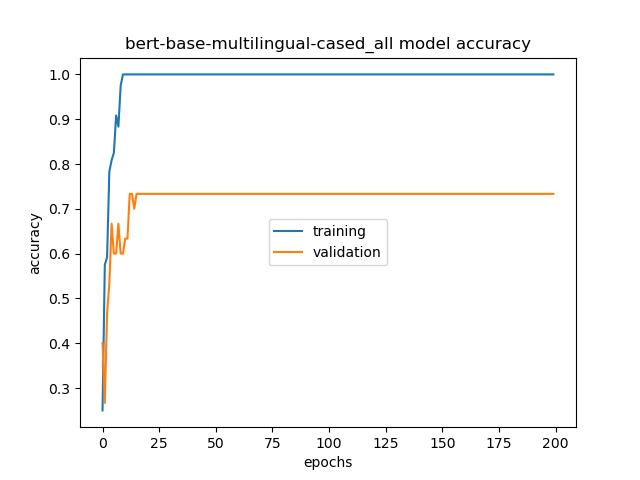
\includegraphics[width=0.49\linewidth,trim={0 0.1cm 0 0},clip]{graphs-newest/webapps_bert-base-multilingual-cased_all-accuracy.png}}
   \caption{Nodomu noteikšanas precizitātes palielināšanās modeļa apmācībās gaitā. Precizitāte aprēķināta uz treniņdatu kopas (zilā līnija) un validācijas datu kopas (oranžā līnija). Izmantota mBERT jēdzientelpa, \textit{Webapps} datu kopa, apmācība notika uz visām valodām, testēšana uz latviešu valodas korpusa (2ab metodes).} 
   \label{fig:webapps-bert-all}
\end{figure}


\begin{figure}[h] 
   \centering
   \subcaptionbox{mBERT angļu treniņdatu kopa}{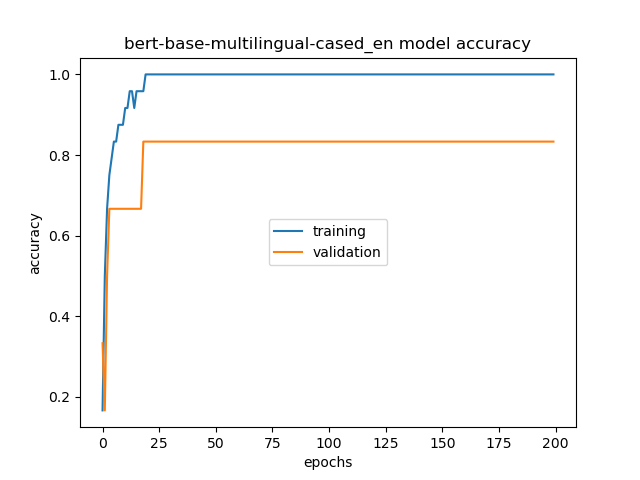
\includegraphics[width=0.49\linewidth,trim={0 0.1cm 0 0},clip]{graphs-newest/webapps_bert-base-multilingual-cased_en-accuracy.png}}
   \subcaptionbox{XLM-RoBERTa angļu treniņdatu kopa}{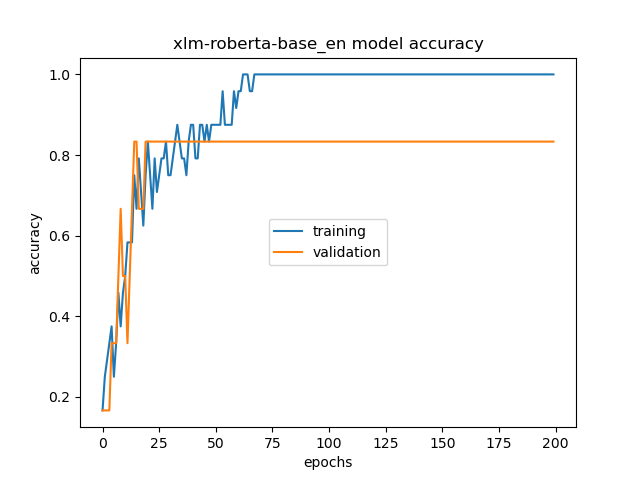
\includegraphics[width=0.49\linewidth,trim={0 0.1cm 0 0},clip]{graphs-newest/webapps_xlm-roberta-base_en-accuracy.png}}
   \caption{Nodomu noteikšanas precizitātes palielināšanās modeļa apmācībās gaitā. Precizitāte tika aprēķināta uz treniņdatu kopas (zilā līnija) un validācijas datu kopas (oranžā līnija). Tika izmantotas dažādas jēdzientelpas, \textit{Webapps} datu kopa, apmācība un testēšana notika uz angļu valodas korpusa (3b metode).} 
   \label{fig:webapps-bert-xlm-en}
\end{figure}


\begin{figure}[h] 
   \centering
   \subcaptionbox{mašīntulkoto latviešu treniņdatu kopa}{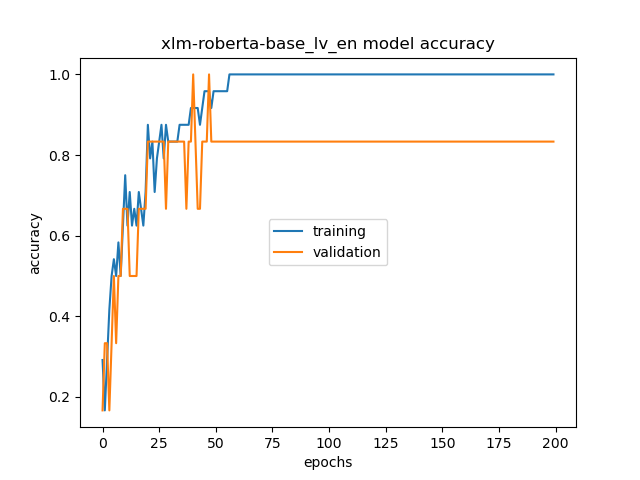
\includegraphics[width=0.49\linewidth,trim={0 0.1cm 0 0},clip]{graphs-newest/webapps_xlm-roberta-base_lv_en-accuracy.png}}
   \subcaptionbox{latviešu treniņdatu kopa}{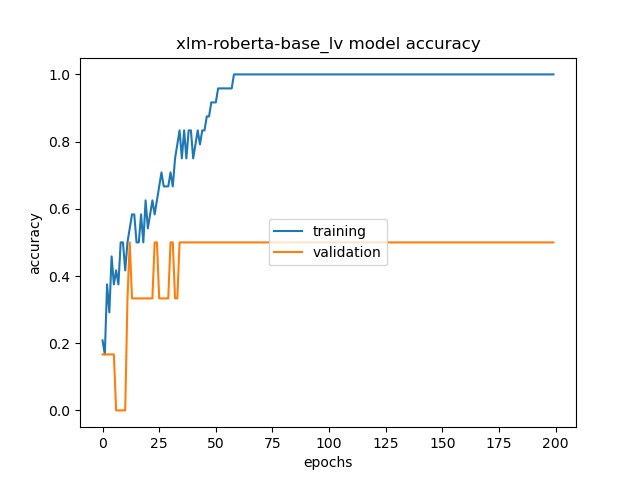
\includegraphics[width=0.49\linewidth,trim={0 0.1cm 0 0},clip]{graphs-newest/webapps_xlm-roberta-base_lv-accuracy.png}}
   \caption{Nodomu noteikšanas precizitātes palielināšanās modeļa apmācībās gaitā. Precizitāte aprēķināta uz treniņdatu kopas (zilā līnija) un validācijas datu kopas (oranžā līnija). Izmantota XLM-RoBERTa jēdzientelpa, \textit{Webapps} datu kopa, apmācība un testēšana notika uz latviešu valodas korpusa (1ab metodes).} 
   \label{fig:webapps-xlm}
\end{figure}


\begin{figure}[h] 
   \centering
   \subcaptionbox{apvienotā mašīntulkoto treniņdatu kopa}{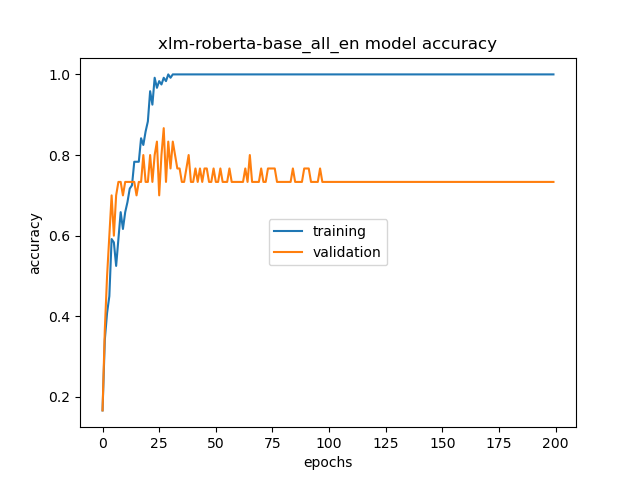
\includegraphics[width=0.49\linewidth,trim={0 0.1cm 0 0},clip]{graphs-newest/webapps_xlm-roberta-base_all_en-accuracy.png}}
   \subcaptionbox{apvienotā treniņdatu kopa}{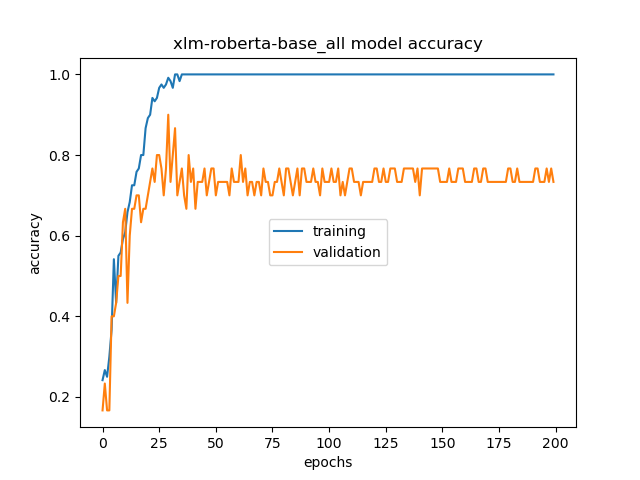
\includegraphics[width=0.49\linewidth,trim={0 0.1cm 0 0},clip]{graphs-newest/webapps_xlm-roberta-base_all-accuracy.png}}
   \caption{Nodomu noteikšanas precizitātes palielināšanās modeļa apmācībās gaitā. Precizitāte aprēķināta uz treniņdatu kopas (zilā līnija) un validācijas datu kopas (oranžā līnija). Izmantota XLM-RoBERTa jēdzientelpa, \textit{Webapps} datu kopa, apmācība notika uz visām valodām, testēšana uz latviešu valodas korpusa (2ab metodes).} 
   \label{fig:webapps-xlm-all}
\end{figure}
